\section{Background}
\paragraph{}
A network/internet measurement platform is an infrastructure of dedicated probes that periodically run network measurement tests on the internet/network\cite{7076582}.

\paragraph{}
 Network measurement platforms from the perspective of end systems normally play an important role both for researchers who want to develop general insight into how the Internet functions, and for general practitioners who want to diagnose individual performance issues \cite{Dhawan:2012:FBN:2398776.2398786}. Use cases of these measurement platforms vary widely based on the type of a user and the end goal of the measurement \cite{Ford:2018:RWR:3243157.3243167}. One example of a use case is how in  previous studies these platforms have been employed to understand the overall network topology of the internet\cite{7076582}.For managers and regulators measurement platforms can provide a different view of the internet e.g routing, topology, addressing and naming, security, dataplane performance or impairment and traffic matrices\cite{Ford:2018:RWR:3243157.3243167}.
\paragraph{}
In some cases measurement platforms are used to detect anomalous behaviour in the network, which could be caused by users abusing the network or general cyber attacks. Internet service providers(ISP) on the other hand use monitoring platforms to evaluate the Quality of Service(QoS) experienced by their users\cite{7076582}. Consumers can also use such measurements to confirm whether the ISP is living up to its Service-Level Agreement(SLA) offers \cite{7076582}.
\paragraph{}
In general measurement platforms are said to provide the engineering to bridge the gap between practice and research\cite{Ford:2018:RWR:3243157.3243167}.
\subsection{Quality Of Service}
Quality of Service(QoS) is about network delivery capacity and resource availability to end-users\cite{5430142}. In other words, one would say QoS is about fast internet access and low latency for the user.
\paragraph{}
However there are many non-uniform views about QoS by different stakeholders. Some say QoS refers to the ability of a network to offer packet transfer in a faster way \cite{5430142}.
\paragraph{}
At the same time other organisations have maintained that QoS has to do with the degree of conformance to user-specified needs \cite{article}. These two different views raise questions of how network level QoS measurements and control relate to the user perception of a service \cite{5430142}.
\paragraph{}
The two main QoS parameters are network latency
and delivery speed(bandwidth) \cite{5430142}. As a result, QoS is considered poor if any of them is affected from their normal position i.e if bandwidth is low or if latency is high.
\subsection{Community Networks}
Community networks are IP-based networks that are built, operated and owned by communities of citizens. These networks are sometimes ran by non-profit organisations working together with local stakeholders in the community\cite{alma990000517660904041}.

Other scholars also define them as large scale, self-organized and decentralized networks, built and operated by citizens for citizens \cite{Braem:2013:CRC:2500098.2500108}.
\paragraph{}
Community networks are normally built as a mixture of both wireless and wired links. This calls for different routing and systems and protocols to be employed in these networks. In some cases there are many wireless links with a limited number of wired links. This makes them predominantly wireless networks\cite{alma990000517660904041}.
\paragraph{}
Providing connectivity to community networks can be a challenging task since nodes use diverse access technologies and display a great deal of mobility \cite{Plagemann2008}.
Due to their non-standard architecture and the use of diverse technology it has proven to be difficult to deploy conventional network measurement platforms on community networks.



\subsection{Introduction}
\paragraph{}
Characterising the internet through measurements has become very important to both end users and network
managers. Most end users want to know what is causing their network based applications to slow down or take too long to respond. On the other hand network managers want to troubleshoot and detect faulty nodes in a network. The rise of cyber attacks and abuse of networks also makes it of paramount importance for network managers to continuously keep track of what is happening in their network.
\paragraph{}
The goal of this paper is to present the design and creation of a visualiser for a quality of service monitoring platform for community networks. Such a visualiser is important in that it can help in monitoring network activity and identifying anomalous behaviour.
\paragraph{}
The platform is built as case study for the iNethi community network at Ocean View, a township in Cape Town. There are two main types of target users for this platform. The first ones are non-technical end-users of the network. These are people who live in the community and use the network for different purposes. The second group are technical(advanced) end-users with a working knowledge of networking protocols. These would include networking researchers from tertiary institutions and network managers.
\paragraph{}
For non-technical users, the goal of the platform is to enable them to get various statistics calculated based on their past network usage. These statistics will also include websites or services which consumes most of their data and the services they visit the most.
\paragraph{}
On the other hand, the goal for technical users, is to allow them run different measurements on the network with the intention to monitor network performance. The results of the measurements are to be displayed on a rich web based visualiser that employs interactive graphs to present each type of measurement. These measurements are to be run on mobile probes deployed on the network. Fig 1 shows how the whole system is to be connected together.

\begin{figure*}
	\centering
	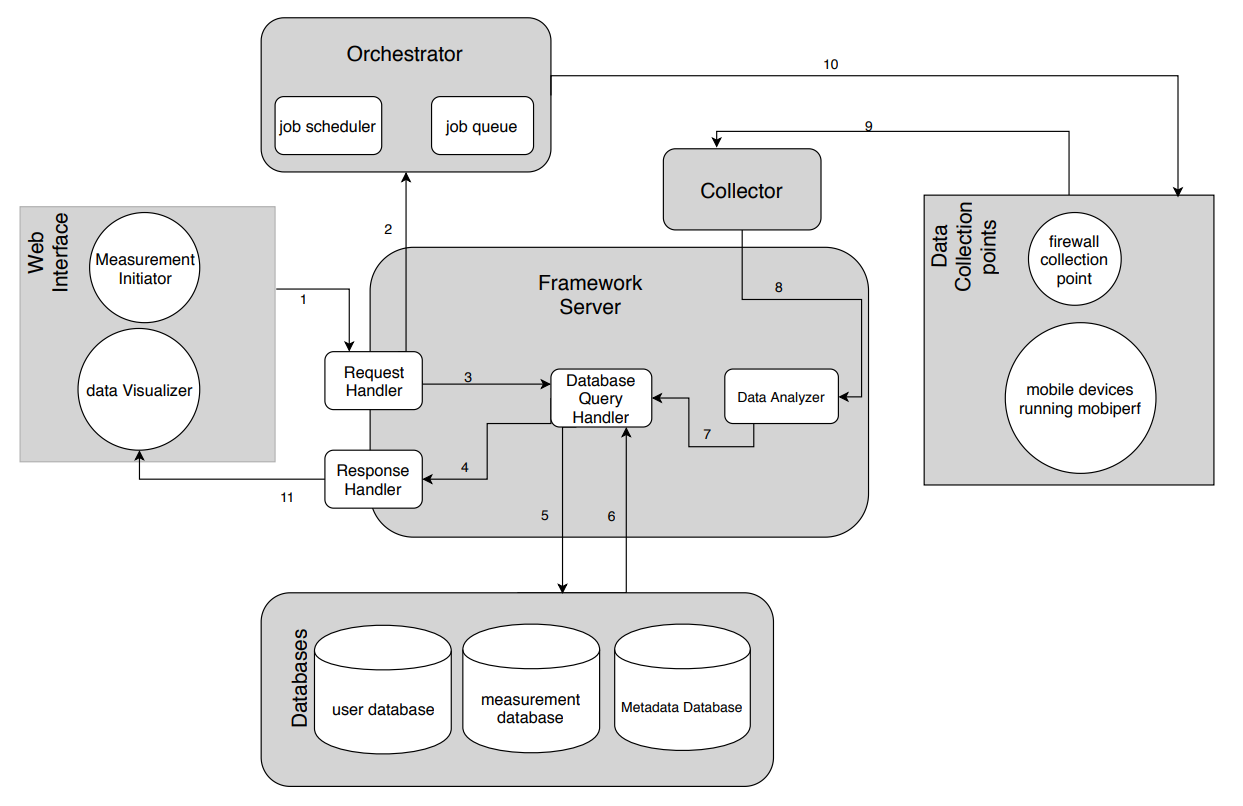
\includegraphics[width=0.7\linewidth]{images/system}
	\caption{Image of the system showing how the visualiser was connected to everything}
	\label{fig:system}
\end{figure*}
